%% Experimental performance
%% 

\section{Performance and Tuning}  

In this section, we report on experiments comparing the tools HPR, BJ and BHKK.  The objective here is to give the reader an indication of the performance that can be expected in practice.  We consider random connected graphs, random planar graphs and random regular graphs.  The machine used for these experiments was an Intel Code i5 3.2GHz with 8GB of memory, running Arch Linux 3.12.9-2.

\subsection{Experimental Procedure}
To generate {\em random connected graphs}, we employed the tool \verb+genrang+ (supplied with {\em nauty}) to construct random graphs with a given number of edges; from these, we selected connected graphs until there were 100 for each value of $|E|$ or $|V|$ (depending upon experiment).  The \verb+genrang+ tool constructs a random graph by generating a random edge, adding it to the graph (if not already present), and then repeating this until enough edges have been added.  We also used \verb+genrang+ to generate random simple regular graphs --- this essentially works by generating a random regular multigraph and then throwing it out if it contains loops or multiple edges.  Generating {\em random planar graphs} required a different approach since the number of randomly generated graphs that are planar is extremely small.  Therefore, we employed a Markov-chain approach:  here, a pair of vertices were selected at random; if the corresponding edge was not already present and the graph would remain planar, then it was added; otherwise, it was removed.  This procedure was repeated for $3n^2$ steps (which, according to \cite{DVW96}, is well beyond the equilibrium point).

\begin{figure}[!p]
\centering
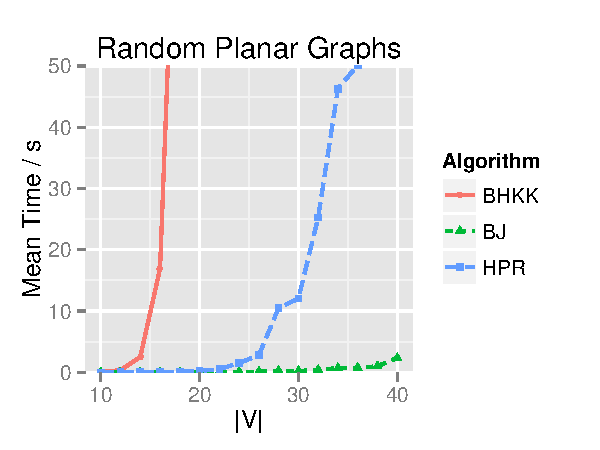
\includegraphics[width=0.5\textwidth]{data/Exp1_planar_graphs.pdf}%
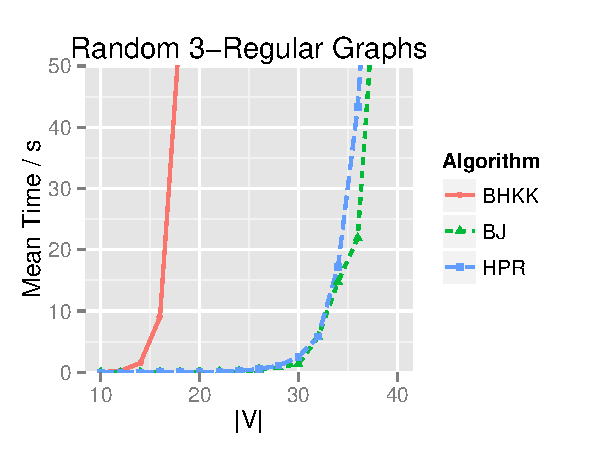
\includegraphics[width=0.5\textwidth]{data/Exp1_reg3_graphs.pdf}
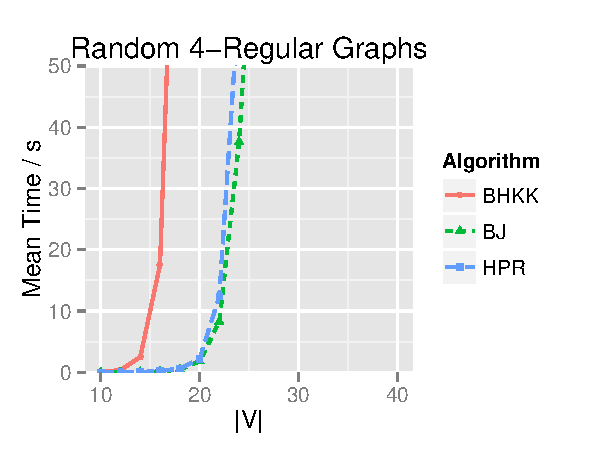
\includegraphics[width=0.5\textwidth]{data/Exp1_reg4_graphs.pdf}%
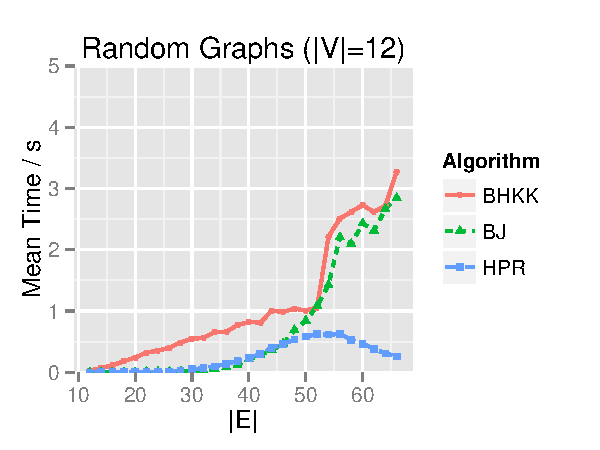
\includegraphics[width=0.5\textwidth]{data/Exp1_random12_graphs.pdf}
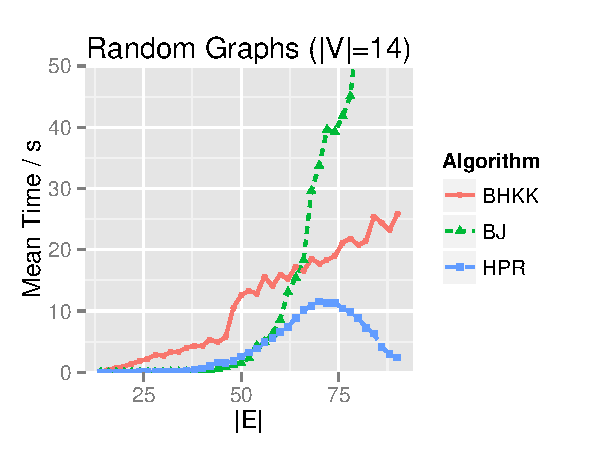
\includegraphics[width=0.5\textwidth]{data/Exp1_random14_graphs.pdf}%
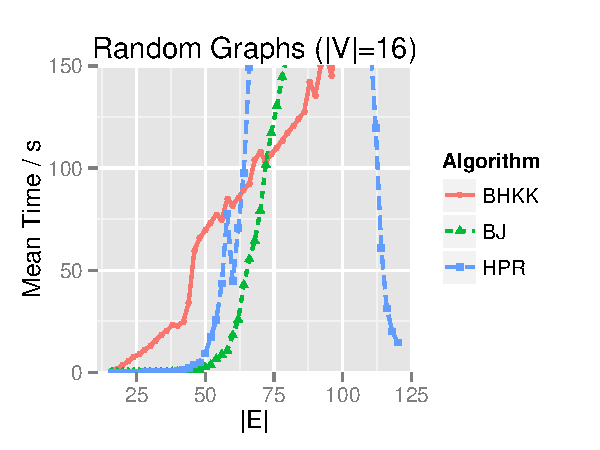
\includegraphics[width=0.5\textwidth]{data/Exp1_random16_graphs.pdf}
\caption{Results from Experiment 1.  Random Planar, 3-Regular and 4-Regular Graphs with varying $|V|$, and random graphs at $|V|= 12$, $|V|= 14$, $|V|= 16$ with varying $|E|$.  Each data-point is averaged over 100 graphs.}
\label{experiment_1}
\end{figure}

\subsection{Experiment I}

In the first experiment, we compared the base performance of the three tools outlined in \S\ref{implementations}.  That is, each tool was executed without any additional command-line parameters being provided.  This gives an out-of-the-box comparison of the tools, and provides a starting point for our subsequent investigations into the effects of the various options available to each tool.

The results from this experiment are shown in Figure~\ref{experiment_1}.  The results show considerable variation between the three tools, with each performing well in some areas.  For example, BHKK performs poorly on sparse graphs, but is more competitive on denser graphs.  Likewise, BJ performs very well on sparse graphs, but poorly on dense graphs. 

An interesting effect can be observed for HPR for the random graphs where $|V|=16$.  Here, we can see a sudden change in the behaviour of the algorithm.  This reflects the edge selection heuristic which, by default, is set to an \verb+auto+ mode.  In this mode the tool examines the graph density and, based on this, switches between a heuristic which operates better on sparse graphs and one which is better for dense graphs.  As we can see, whilst this mode is having a useful effect, it is also far from optimal.

\subsection{Experiment 2}
Another important parameter for tuning the HPR tool is the choice of {\em edge selection heuristic} (see~\cite{PHR09} for more on this).  By default, the HPR tool attempts to pick the appropriate heuristic based on density of the input graph.  As highlighted already, this is often inadequate and, in our second experiment, we examine the effect of this on performance of the HPR tool.  This was done by running the tool with three different command-line options for manipulating the edge-selection heuristic:

\begin{itemize}
\item \verb+--sparse+.  With this command-line option the edge selection heuristic is fixed at the \verb+minsdeg+ heuristic of Pearce {\em et al.}~\cite{PHR09}.  This selects an arbitrary edge to delete / contract from those with an end-point of minimal degree compared with any vertex in the graph.
\item \verb+--dense+.  With this command-line option the edge selection heuristic is fixed at the \verb+vorder+ heuristic of Pearce {\em et al.}~\cite{PHR09} (also referred to as \verb+vorder-pull+ by Monagan~\cite{Mon12}).  In this heuristic, the vertices of the graph are given a fixed, predefined ordering. Then, as the computation proceeds, edges are selected from the lowest vertex in the order until it becomes disconnected
\item {\em Default}.  A default \verb+auto+ mode for the HPR tool is used when no specific option is given directing the edge selection heuristic.  In this mode, the algorithm chooses the heuristic given by \verb+--vorder-push+ for sparse graphs and \verb+--dense+ for dense graphs.  The former was described by Monagan~\cite{Mon12}.  
\end{itemize}

The results from this experiment are shown in Figure~\ref{experiment_2}.  The data shows that the \verb+--sparse+ and \verb+--dense+ do work well in their target area.  However, it is perhaps surprising that \verb+--sparse+ does not perform better on the random 3-regular graphs.  Finally, the default mode is never optimal, but does generally provide competitive behaviour.  Again, we can see distinctly the areas where the default mode switches from one heuristic to another.

\begin{figure}[!p]
\centering
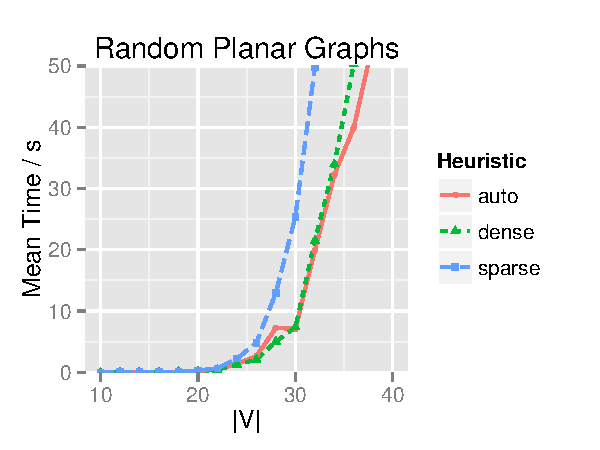
\includegraphics[width=0.5\textwidth]{data/Exp2_planar_graphs.pdf}%
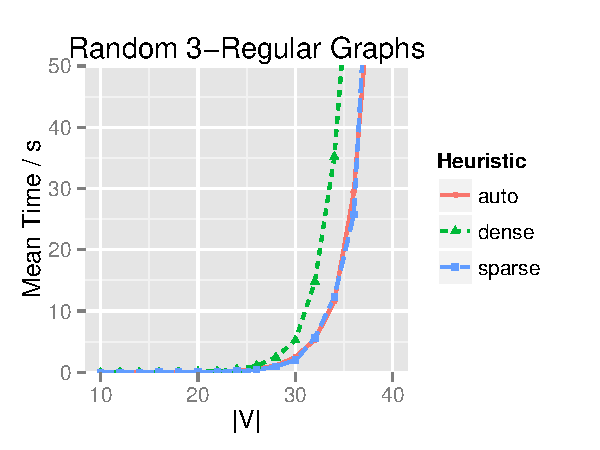
\includegraphics[width=0.5\textwidth]{data/Exp2_reg3_graphs.pdf}
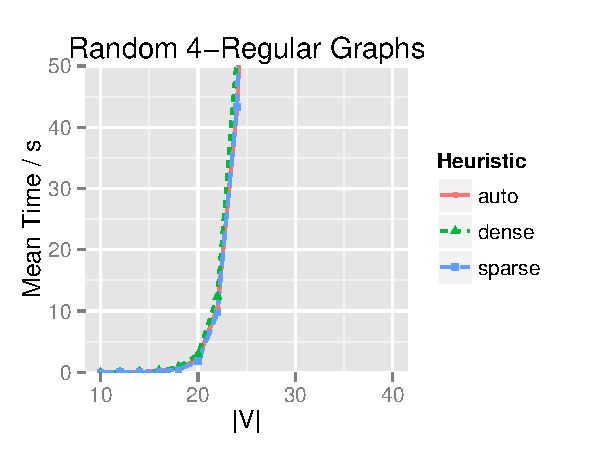
\includegraphics[width=0.5\textwidth]{data/Exp2_reg4_graphs.pdf}%
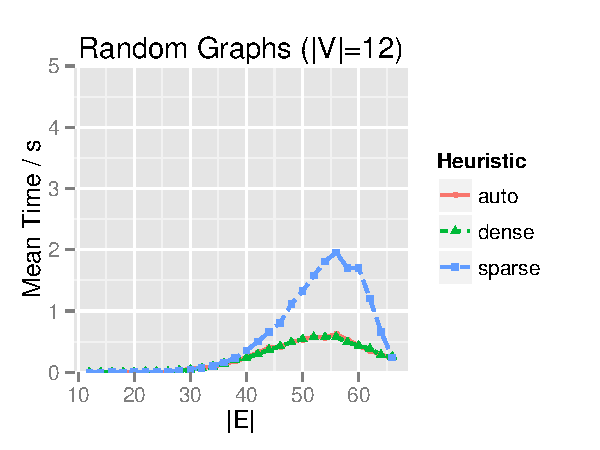
\includegraphics[width=0.5\textwidth]{data/Exp2_random12_graphs.pdf}
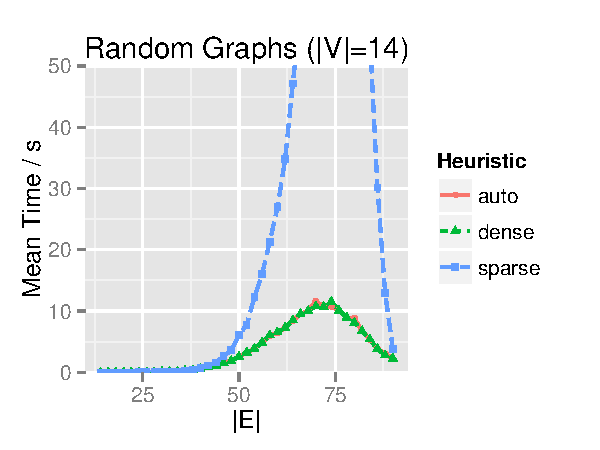
\includegraphics[width=0.5\textwidth]{data/Exp2_random14_graphs.pdf}%
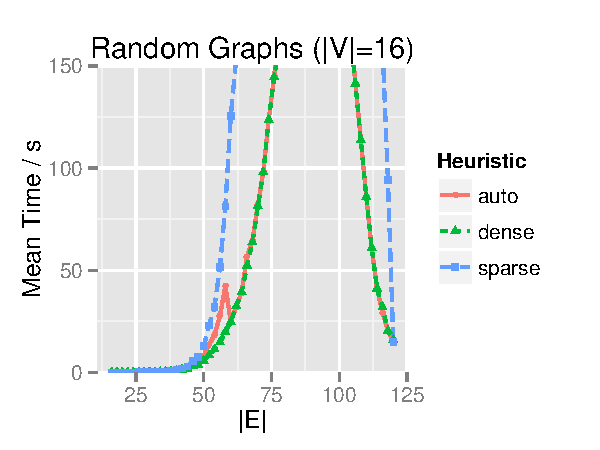
\includegraphics[width=0.5\textwidth]{data/Exp2_random16_graphs.pdf}
\caption{Results from Experiment 2.  Random Planar, 3-Regular and 4-Regular Graphs with varying $|V|$, and random graphs at $|V|= 12$, $|V|= 14$, $|V|= 16$ with varying $|E|$.  Each data-point is averaged over 100 graphs.}
\label{experiment_2}
\end{figure}



\subsection{Experiment 3}
 
A critical parameter for tuning the HPR tool is the amount of RAM used for the cache of previously computed graphs.  This is adjusted using the \verb+--cache-size=X+ command-line option.  If this option is not given (as for Experiment 1), then 256MB is set aside by default.  In our experience, this can be woefully inadequate for large graphs.  Therefore, in our third experiment, we examined the effect of cache size on performance of the HPR tool.  This was done by running the tool with varying cache sizes over the same set of graphs as before.

The results from this experiment are shown in Figure~\ref{experiment_3}.  The results show limited benefit from the use of large cache sizes, although it is clear that larger graphs show more benefit.  Indeed, our experience in tackling very large graphs (e.g. the Truncated Icosahedron~\cite{HPR10}) choosing the largest possible cache size which fits within available RAM is critical.  For example, we routinely use machines with 64GB of RAM for handling large graphs.

\begin{figure}[!p]
\centering
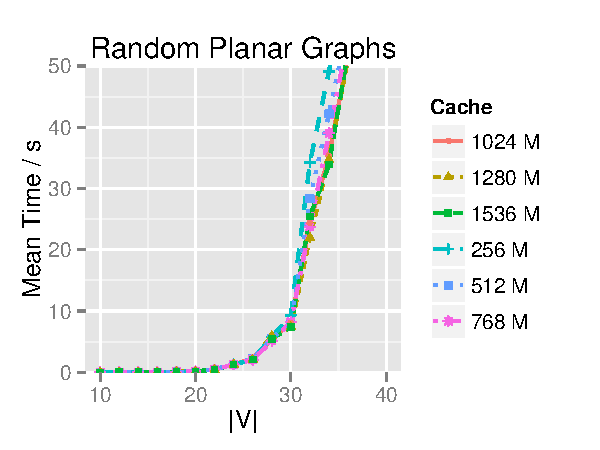
\includegraphics[width=0.5\textwidth]{data/Exp3_planar_graphs.pdf}%
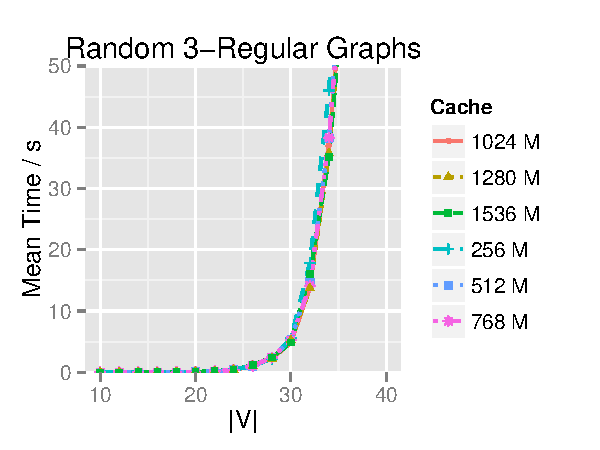
\includegraphics[width=0.5\textwidth]{data/Exp3_reg3_graphs.pdf}
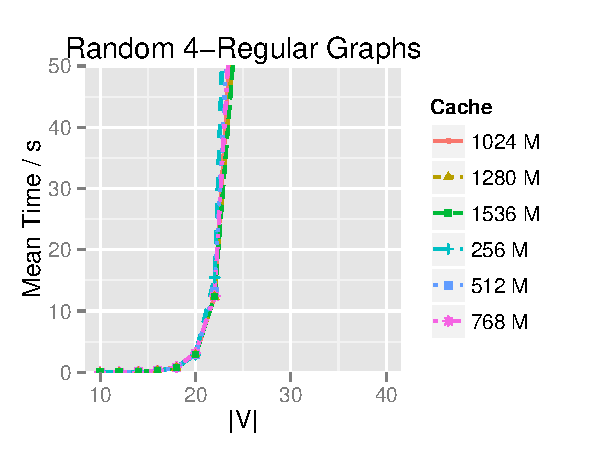
\includegraphics[width=0.5\textwidth]{data/Exp3_reg4_graphs.pdf}%
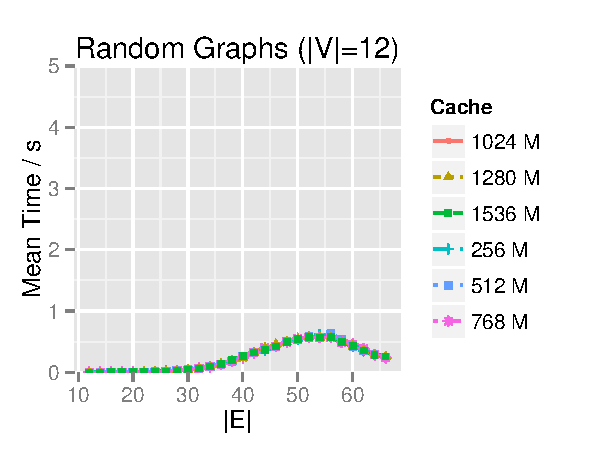
\includegraphics[width=0.5\textwidth]{data/Exp3_random12_graphs.pdf}
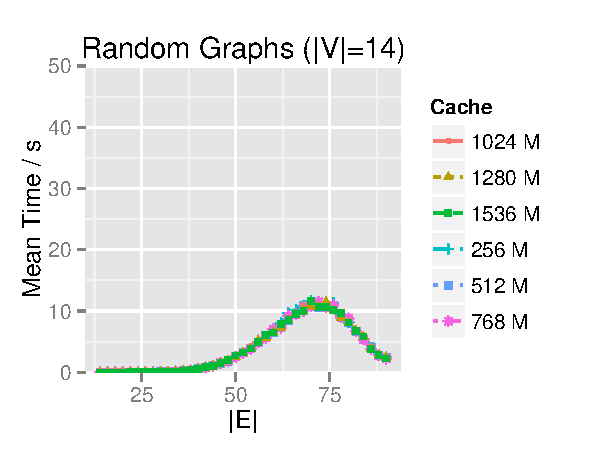
\includegraphics[width=0.5\textwidth]{data/Exp3_random14_graphs.pdf}%
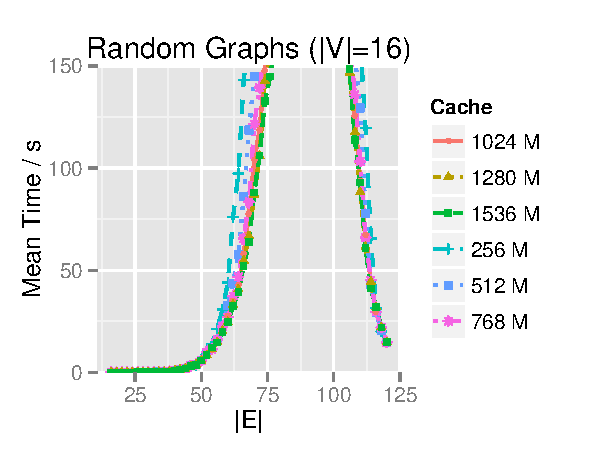
\includegraphics[width=0.5\textwidth]{data/Exp3_random16_graphs.pdf}
\caption{Results from Experiment 3.  Random Planar, 3-Regular and 4-Regular Graphs with varying $|V|$, and random graphs at $|V|= 12$, $|V|= 14$, $|V|= 16$ with varying $|E|$.  Each data-point is averaged over 100 graphs.}
\label{experiment_3}
\end{figure}
